%----------------------------------------------------------------------
% Longueur : 1 page maximum
\subsection{Réseau de neurones (MLP)}
\responsable{Thibault}

\paragraph{Principe.}
Nous utilisons un perceptron à \textbf{une couche cachée}, suffisante en principe d'après le théorème
d'approximation universelle, qui ne dit rien en revanche du nombre de neurones nécessaire :
\begin{equation}
\hat{v}_i(t+h)=\bm{w}_2\tr\tanh\!\bigl(\bm{W}_1\bm{x}_i(t)+\bm{b}_1\bigr)+b_2 .
\end{equation}
Les 30 neurones cachés $\tanh$ apportent la non-linéarité ; la sortie est linéaire, car la grandeur prédite ne
doit pas être bornée. Le même réseau sert aux 36 capteurs, avec des entrées centrées-réduites. Les poids
minimisent l'erreur quadratique par rétropropagation (Adam, scikit-learn). Le problème n'étant pas convexe, chaque
configuration est entraînée avec 5 graines. L'\emph{early stopping} s'arrête quand le score sur 10\,\% des exemples
mis de côté stagne ; la tolérance par défaut l'arrêtait trop tôt, d'où une patience de 30 époques.

Trois variantes sont testées. \texttt{spatial} ajoute la moyenne des 10 débits passés des voisins dans $\bm{A}$
(58 entrées, soit $59\times30+31=1\,801$ paramètres pour environ 36\,000 exemples). \texttt{variation} fait
apprendre $v_i(t+1)-v_i(t)$, ce que la persistance ne sait pas prédire. L'\emph{ensemble} moyenne les
prédictions des 5 réseaux, sur le principe du bagging.

\begin{center}
\small
\begin{tabular}{lcc}
\toprule
Validation, $h=1$, 30 neurones $\tanh$ & Un réseau (moy.\ $\pm$ é.-t.) & Ensemble des 5 \\
\midrule
Persistance & \multicolumn{2}{c}{0,0381} \\
base, débit & 0,0316 $\pm$ 0,0004 & 0,0304 \\
base, variation & 0,0314 $\pm$ 0,0002 & 0,0303 \\
spatial, débit & 0,0310 $\pm$ 0,0001 & 0,0298 \\
\textbf{spatial, variation} & \textbf{0,0309} $\pm$ 0,0001 & \textbf{0,0299} \\
\bottomrule
\end{tabular}

\vspace{0.6em}
\begin{tabular}{lcccc}
\toprule
Spatial, variation & \multicolumn{4}{c}{Neurones dans la couche cachée} \\
\cmidrule(lr){2-5}
(validation, $h=1$) & 10 & 30 & 50 & 100 \\
\midrule
$\tanh$, un réseau & 0,0311 $\pm$ 0,0004 & 0,0309 $\pm$ 0,0001 & 0,0308 $\pm$ 0,0003 & 0,0312 $\pm$ 0,0004 \\
$\tanh$, ensemble  & 0,0302 & 0,0299 & \textbf{0,0297} & 0,0300 \\
ReLU, un réseau    & 0,0316 $\pm$ 0,0004 & 0,0314 $\pm$ 0,0001 & 0,0316 $\pm$ 0,0002 & 0,0319 $\pm$ 0,0006 \\
ReLU, ensemble     & 0,0306 & 0,0303 & 0,0305 & 0,0304 \\
\bottomrule
\end{tabular}
\end{center}

\begin{figure}[ht]
\centering
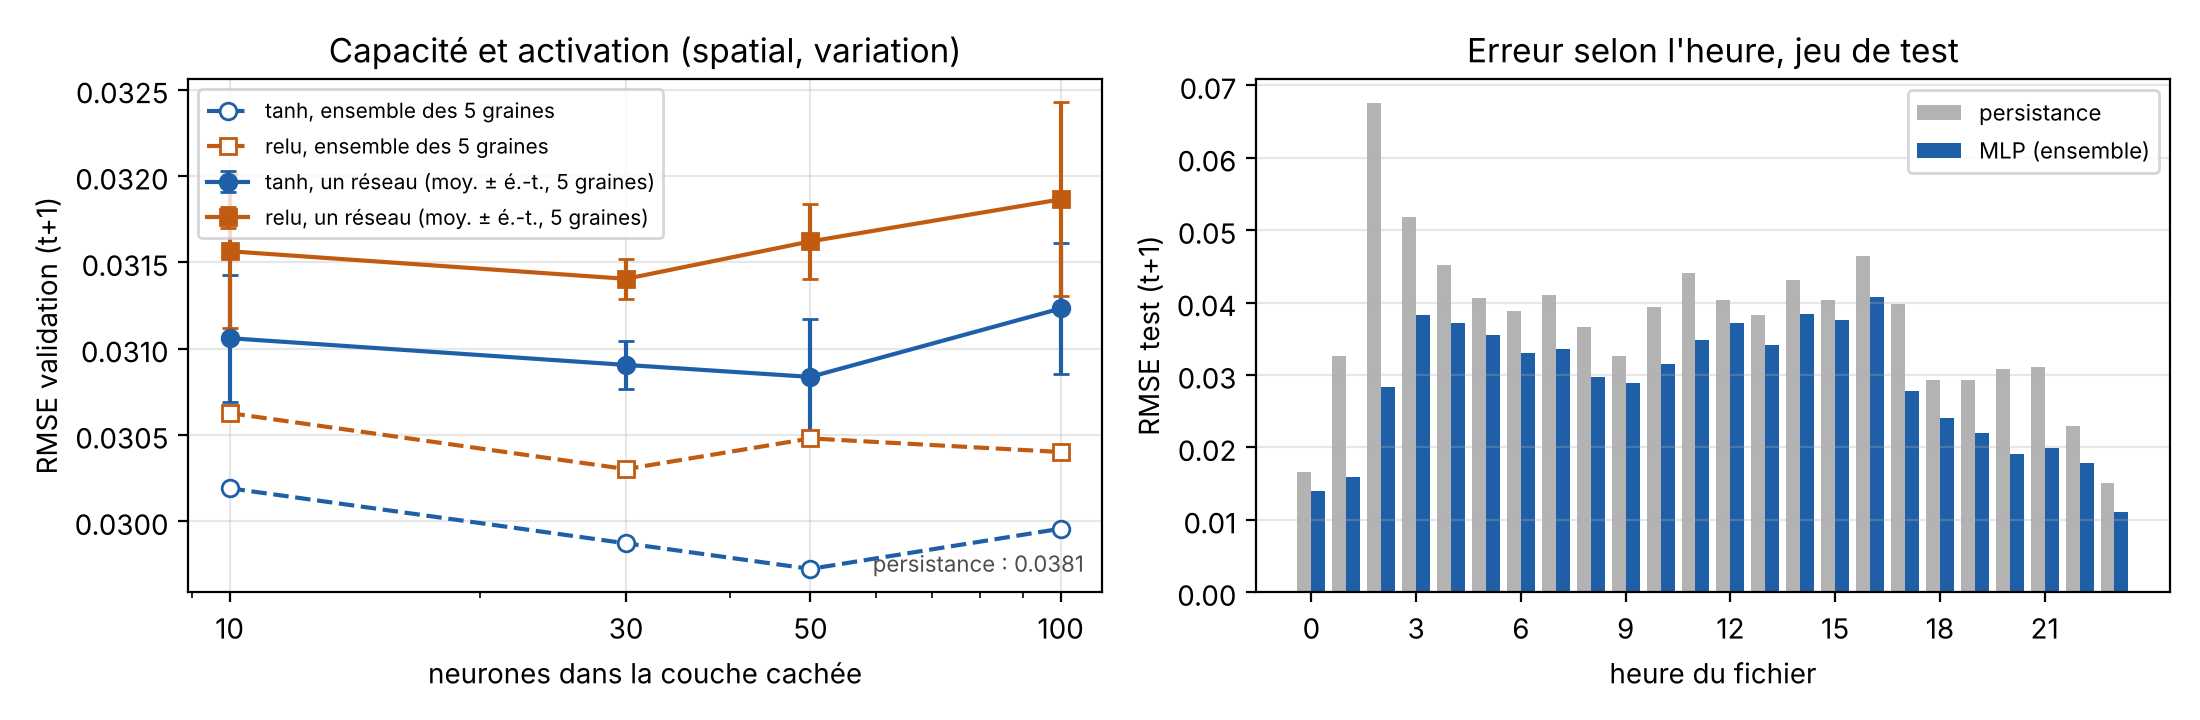
\includegraphics[width=0.8\linewidth]{figures/mlp.png}
\caption{À gauche : RMSE de validation selon le nombre de neurones et l'activation (traits pleins : un réseau,
moyenne et écart-type sur 5 graines ; pointillés : ensemble). À droite : erreur de test par heure du fichier.}
\label{fig:mlp}
\end{figure}

\paragraph{Analyse.}
\begin{itemize}
  \item \textbf{L'ensemble apporte plus que les réglages.} \texttt{spatial} et \texttt{variation} gagnent quelques
  $10^{-4}$, du même ordre que la dispersion entre graines : sur 2,6 jours de validation, ce n'est pas significatif.
  Moyenner 5 réseaux gagne environ 0,001 dans toutes les configurations : agréger des modèles qui se trompent
  différemment réduit la variance, comme pour la forêt aléatoire.
  \item \textbf{La capacité compte peu} entre 10 et 100 neurones (figure~\ref{fig:mlp}), l'\emph{early stopping}
  limitant le surapprentissage. $\tanh$ bat systématiquement ReLU, cohérent avec des entrées centrées et une
  variation à prédire symétrique.
  \item \textbf{Le gain se concentre lors des changements rapides} : $-50$ à $-58\,\%$ d'erreur par rapport à la
  persistance aux heures 1 et 2 du fichier, quand le trafic monte brusquement, contre $-7$ à $-11\,\%$ en milieu de
  journée. C'est là que la non-linéarité sert.
  \item \textbf{Sur le test}, l'ensemble retenu (spatial, variation, réentraîné sur entraînement + validation) obtient
  0,0302 à 15 minutes (MAE 0,0205, $-22\,\%$ par rapport à la persistance) et, sans nouveau réglage, 0,0348 à
  30 minutes (MAE 0,0235, $-36\,\%$). Sur cette cible et ce test, l'article annonce 0,0448 pour sa meilleure
  méthode, linéaire~\cite{zhao2019}.
\end{itemize}
\textbf{Limites.} Chaque couple (instant, capteur) est traité indépendamment : l'historique n'est vu qu'à travers
10 retards et le réseau routier qu'à travers une moyenne des voisins. Le modèle est aussi peu lisible ; un réseau
récurrent ou sur graphe exploiterait mieux ces structures, avec plus de données.
